\documentclass[]{exam}
\usepackage{epic,array,ecltree,url,calrsfs}
\usepackage[nointegrals]{wasysym}

%These tell TeX which packages to use.
\usepackage{array,epsfig}
\usepackage{amsmath}
\usepackage{amsfonts}
\usepackage{amssymb}
\usepackage{amsxtra}
\usepackage{amsthm}
\usepackage{mlextra} % must come after ams packages
\usepackage{mathrsfs}
\usepackage[dvipsnames]{xcolor}
\usepackage{array}
\usepackage{graphicx}
\graphicspath{ {../art/} }
\usepackage{subfig}
\usepackage{bm}
\usepackage{tikz}
\usepackage{multicol}
\usepackage{enumitem}

\newcommand{\twonode}{%
  \begingroup\normalfont
  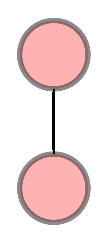
\includegraphics[height=\fontcharht\font`\b]{2nodetree.eps}%
  \endgroup
}

\newcommand{\tf}[1][{}]{%
\fillin[#1][0.25in]%
}
\title{Lab 9: Introduction to Temporal Logic}
\author{Foundations of Computer Science}
\date{\today}
%\pagestyle{empty} 
%\footer{}{\thepage}{}
\unframedsolutions
\SolutionEmphasis{\itshape\small}
\SolutionEmphasis{\color{NavyBlue}}


\begin{document}

\maketitle
\setlength{\columnseprule}{1pt}
\begin{questions} 


\question Define propositions $p$ and $q$ as follows:\\
$p$:``The light is green''\\
$q$: ``The light is red.''\\
Express the following in linear temporal logic:
\begin{parts}
\part The light is always eventually green.
\vspace{5mm}
\begin{solution}
$\Box \Diamond p$
\end{solution}

\part A red light never immediately follows a green light.
\vspace{5mm}
\begin{solution}
$\Box (p \imp \ngg \Circle q)$
\end{solution}

\part The light is never both red and green at the same time.
\vspace{5mm}
\begin{solution}
$\Box (\ngg p \lor \ngg q)$
\end{solution}

\part It is always the case that a red light is eventually not red.
\vspace{5mm}
\begin{solution}
$\Box (q \imp \Diamond \ngg q)$
\end{solution}
\end{parts}

\question Define propositions $p$, $q$, $r$ and $s$ as follows:\\
 $p$: ``The job is requested.''\\
 $q$: ``The request is received.''\\ 
 $r$: ``The request is processed.''\\
 $s$: ``The request is completed.''\\
Express the following in linear temporal logic:
\begin{parts}
\part It is always the case that if a job is requested it is eventually
received.
\vspace{5mm}
\begin{solution}
$\Box (p \imp \Diamond q)$
\end{solution}

\part It is always the case that if a job is received it will be processed next.
\vspace{5mm}
\begin{solution}
$\Box (q \imp \Circle r)$
\end{solution}

\part It is always the case that if a job is processed it will eventually be
always completed.
\vspace{5mm}
\begin{solution}
$\Box (r \imp \Diamond \Box s)$
\end{solution}
\end{parts}

\question Define propositions $p$, $q$, $p'$ and $q'$ as follows:\\
 $p$: ``Process p is in the critical section.''\\
 $q$: ``Process q is in the critical section.''\\ 
 $p'$: ``Process p is attempting to enter the critical section.\\
 $q'$: ``Process q is attempting to enter the critical section.''\\
Express the following desirable properties of a concurrent system:
\begin{parts}
\part Process $p$ and process $q$ cannot both be
in the critical section at the same time. (mutual exclusion)
\vspace{5mm}
\begin{solution}
$\Box \ngg (p \land q)$
\end{solution}

\part If a process attempts to enter its critical section, it
will eventually succeed. (liveness)
\vspace{5mm}
\begin{solution}
$\Box (p' \imp \Diamond p) \land \Box (q' \imp \Diamond q)$
\end{solution}

\part It is always the case that if a process is in the critical
section it eventually leaves the critical section.
\vspace{5mm}
\begin{solution}
$\Box (p \imp \Diamond \ngg p) \land \Box (q \imp \Diamond \ngg q)$
\end{solution}
\end{parts}


\question Convert the following from first order logic to temporal logic.
Assume $g(x,y)$ is interpreted as the $\geq$ relation. All other relations
have arbitrary assignments.
\begin{parts}
\part $\forall t \ngg q(t)$
\vspace{5mm}
\begin{solution}
$\Box \ngg p$
\end{solution}

\part $\forall t_1 (r(t_1) \imp \exists t_2 (g(t_2, t_1) \land z(t_2)))$.
\vspace{5mm}
\begin{solution}
$\Box (r \imp \Diamond z)$
\end{solution}

\end{parts}

\question Evaluate the following statements with respect to the transition
diagram given.
\begin{parts}
\part Assume $p$ and $q$ continue to alternate.\\
\unitlength=.9pt
\begin{picture}(340,30)
\put(  0, 0){\state{$p$}{$s_{0}$}}
\put( 20,10){\vector(1,0){40}}
\put( 60, 0){\state{$q$}{$s_{1}$}}
\put( 80,10){\vector(1,0){40}}
\put(120, 0){\state{$p$}{$s_{2}$}}
\put(140,10){\vector(1,0){40}}
\put(180, 0){\state{$q$}{$s_{3}$}}
\put(200,10){\vector(1,0){40}}
\put(240, 0){\state{$p$}{$s_{4}$}}
\put(260,10){\vector(1,0){40}}
\put(300, 5){\makebox(20,10){\ldots}}
\end{picture}

\begin{multicols}{2}
\begin{subparts}
\subpart \tf[T] (T/F) $s_0 \models \Diamond p$ 
\subpart \tf[F] (T/F) $s_0 \models \Box p$ 
\subpart \tf[T] (T/F) $s_0 \models \Box \Diamond p$ 
\subpart \tf[F] (T/F) $s_0 \models \Diamond \Box p$ 
\subpart \tf[T] (T/F) $s_0 \models \Diamond p \land \Diamond q$ 
\subpart \tf[F] (T/F) $s_0 \models \Diamond (p \land q)$

\subpart \tf[T] (T/F) $\models \Circle p \eqv \ngg \Circle \ngg p$ 
\subpart \tf[T] (T/F) $\models \Circle p \imp \Diamond p$ 
\subpart \tf[F] (T/F) $ \models \Box (p \lor q) \imp (\Box p \lor \Box q)$ 
\subpart \tf[T] (T/F) $\models \Diamond \Diamond q \eqv \Diamond q$ 
\subpart \tf[T] (T/F) $\models \Diamond \Box \Diamond q \eqv \Box \Diamond q$ 
\subpart \tf[F] (T/F) $\models (\Box \Diamond p \land \Box \Diamond q) \imp \Box \Diamond (p \land q)$
\end{subparts}
\end{multicols}

\vspace{4mm}
\part Assume all states after $s_4$ are labeled $p$.\\ 
\unitlength=.9pt
\begin{picture}(340,30)
\put(  0, 0){\state{$q$}{$s_{0}$}}
\put( 20,10){\vector(1,0){40}}
\put( 60, 0){\state{$q$}{$s_{1}$}}
\put( 80,10){\vector(1,0){40}}
\put(120, 0){\state{$p$}{$s_{2}$}}
\put(140,10){\vector(1,0){40}}
\put(180, 0){\state{$p$}{$s_{3}$}}
\put(200,10){\vector(1,0){40}}
\put(240, 0){\state{$p$}{$s_{4}$}}
\put(260,10){\vector(1,0){40}}
\put(300, 5){\makebox(20,10){\ldots}}
\end{picture}
\begin{multicols}{2}
\begin{subparts}
\subpart \tf[F] (T/F) $s_2 \models \Diamond q$ 
\subpart \tf[F] (T/F) $s_0 \models \Box p$ 
\subpart \tf[T] (T/F) $s_0 \models \Box \Diamond p$ 
\subpart \tf[T] (T/F) $s_0 \models \Diamond \Box p$ 
\subpart \tf[T] (T/F) $s_1 \models \Box \Circle p$ 
\subpart \tf[T] (T/F) $s_1 \models \Circle \Box p$ 

\subpart \tf[T] (T/F) $ \models \Box p \imp \Circle p$ 
\subpart \tf[T] (T/F) $ \models \Diamond \Box p \imp \Box \Diamond p$ 
\subpart \tf[T] (T/F) $ \models \Box p \eqv p \land \Circle \Box p$ 
\subpart \tf[T] (T/F) $ \models \Diamond \Circle q \eqv \Circle \Diamond q$ 
\subpart \tf[T] (T/F) $ \models \Diamond q \eqv q \lor \Circle \Diamond q$ 
\subpart \tf[T] (T/F) $ \models \Box (p \imp \Circle p) \imp (p \imp \Box p)$ 
\end{subparts}
\end{multicols}
\end{parts}

\vspace{4mm}
\question Repeat the same exercise, but assume $\Box$ and $\Diamond$ are evaluated 
directly on $\rho$, rather than the reflexive, transitive closure of $\rho$
(the definition Ben Ari gives in 13.2.2).
\begin{multicols}{2}
\begin{subparts}
\subpart \tf[T] (T/F) $s_0 \models \Diamond p$ 
\subpart \tf[T] (T/F) $s_0 \models \Box q$ 
\subpart \tf[F] (T/F) $s_1 \models \Box q$ 
\subpart \tf[T] (T/F) $s_0 \models \Diamond \Box q$ 
\subpart \tf[F] (T/F) $s_2 \models \Diamond \Box q$ 
\subpart \tf[T] (T/F) $s_0 \models \Box \Diamond q$ 
\subpart \tf[T] (T/F) $s_i \models \Box \Diamond q$ for $i \in \{0,1,2,3\}$ 
\subpart \tf[T] (T/F) $s_0 \models \Diamond \Box (p \land q) $ 
\subpart \tf[T] (T/F) $s_1 \models \Diamond \Diamond \Box (p \land q) $ 
\subpart \tf[F] (T/F) $s_i \models \Diamond \Box (p \land q)$ for $i \in \{0,1,2,3\}$   
\end{subparts}

\unitlength=1.3pt
\begin{picture}(140,105)
\put(0,60){
  \put(10,10){\state{$p$}{$s_{0}$}}
  \put(30,20){\vector(1,0){39}}
  \put(70,10){\state{\shortstack{$p$\\$q$}}{$s_{1}$}}
  \put(77, 9){\line(0,-1){4}}
  \put(65, 7){\oval(24,12)[b]}
  \put(65, 7){\oval(24,12)[tl]}
  \put(64,13){\vector(1,0){8}}
  \put(89,25){\vector(1,0){41}}
  \put(131,15){\vector(-1,0){41}}
  \put(130,10){\state{$q$}{$s_{2}$}}
  \put(127,35){\oval(26,20)[tr]}
  \put(127,45){\line(-1,0){94}}
  \put(33, 35){\oval(27,20)[tl]}
  \put(140,33){\vector(0,-1){0}}
}
\put(70,0){
\put(0,10){\state{}{$s_{3}$}}
\put(10, 9){\line(0,-1){3}}
\put(22, 7){\oval(24,12)[b]}
\put(22, 7){\oval(24,12)[tr]}
\put(24,13){\vector(-1,0){6}}
\put(10,69){\vector(0,-1){38}}
\put(18,28){\vector(1,1){44}}
}
\end{picture}


\end{multicols}

\end{questions}
\end{document}


